\documentclass[UTF8,a4paper,11pt]{ctexart}
\usepackage[margin=22mm]{geometry}
\usepackage{graphicx,hyperref,longtable,booktabs}
\begin{document}
\title{基于 DiTing 的早期 PGA 概率预测}\maketitle

作者、单位和通讯作者待作者确认。本文为供科学审阅的中文首稿。

\section*{摘要}

利用地震发生初期的有限观测预测其他台站的峰值地面加速度，是地震预警的重要任务。本文将冻结的 DiTing 波形编码器接入统一的坐标查询和概率读出框架，在日本 K-NET 事件划分的验证集上，与采用 PhaseNet、EQTransformer 和从头训练 TEAM 波形前端的完整模型比较。四种模型均保留物理幅值和有效观测时长，以首个 P 波到达后的共同截止时间评价非输入目标，并分别分析空间质量与交付时钟。在种子 42、按验证集选择的检查点下，1310 个事件的 139440 条非输入目标请求中，DiTing 的等单元 MAE 为 0.222859 dex，PhaseNet 为 0.225697 dex；首秒差值为 −0.009990 dex，事件聚类自助法 95\% 区间为 [−0.015231，−0.004792] dex。概率评分改善同时伴随欠覆盖，DiTing 的名义 95\% 区间实际覆盖率为 91.49\%。固定目标逐秒回放进一步表明，在 normal 几何下 207 个适格 never-input 事件中，0.20 dex 场质量预算的 20 秒内确认数，DiTing 与 PhaseNet 从理想时钟的 88 与 73，降至数值时钟的 49 与 69，以及含渲染时钟的 15 与 16。结果支持 DiTing 对早期非输入台站预测的有限增益，同时显示校准、人口支持和交付成本共同限制其应用。本文证据属于单种子验证集比较，不构成独立测试或实时部署认证。

全部 PGA 指标使用 log10(m/s²) 坐标，空间场、逐目标请求与固定目标事件分别采用各自的支持分母。既有分层中单输入台站和部分未触发目标未呈现一致改善，全部预设告警阈值亦显示失败与误报之间的权衡。研究为后续独立校准和资源一致的交付验证提供了可追溯依据。

关键词：地震预警；峰值地面加速度；DiTing；概率预测；非输入台站；交付时延

\section*{1 引言}

地震预警需要在破坏性地震动到达前，为不同位置提供可采取行动的信息。预测震级与震源位置能够描述事件，却不能直接回答某一目标点将经历多大的地面运动。峰值地面加速度（PGA）为这个问题提供了明确的物理量；其预测还必须面对观测前缀短、输入台站不断增加以及传播路径和场地差异等困难。预警价值因此同时取决于预测误差、概率可信程度和信息抵达目标用户的时间。只比较最终观测充分时的回归精度，无法完整评价地震初期的使用条件。

直接从波形学习地震动预测，可以减少显式震源反演与经验衰减关系之间的串联误差。TEAM 将多台站波形和位置表示组合起来，对任意查询位置输出地震动分布，为网络式预测提供了代表性框架（Münchmeyer 等，2021）。PhaseNet 与 EQTransformer 则主要面向震相拾取和事件检测，说明波形表征能够从大规模有标签地震记录中学习（Zhu 和 Beroza，2019；Mousavi 等，2020）。把这些前端接入 PGA 任务，需要重新训练任务适配和读出部分，不能把原论文的检测能力直接视为地震动预测能力。

近期单台站 PGA 研究继续探索不同波形网络与不确定性表达。例如 ConvMixer 被用于由早期波形预测对应台站的 PGA（Mohammed 等，2025），共形预测研究则关注短波形区间的覆盖与误报权衡（Shin 和 Jeong，2026）。这些工作与跨台站查询共享早期信息不足的问题，但输入、目标人口、数据划分及评价坐标不同，文献间数值不能直接排名。尤其是已经向模型提供波形的目标和完全未提供波形的目标，所包含的预测难度不同，二者混合后的平均误差可能掩盖外推不足。

DiTing 波形编码器为迁移丰富表征到下游地震动任务提供了另一条路径。本研究关注一个可检验的问题：在统一监督任务、相同事件划分和共同观测截止时间下，采用 DiTing 的完整模型是否能更好地预测非输入台站的 PGA 分布。本文使用的具体编码器由归档资产与校验值界定。其精确预训练语料和对应公开模型论文尚未核实，因此本文不以模型名称推断训练数据，也不把结果解释为预训练机制的单独因果效应。

本文从点预测、概率预测、空间质量和交付四个方面回答上述问题。首先保留历史五个共同截止时点的配对预测，分别报告全部目标和逐时点非输入目标。随后使用已有的固定查询逐秒回放，区分理想截止、完整数值计算和包含比较图渲染的交付时钟。最后将预警失败的未知界限与完整观测负例的误报率同时展示。整个分析只读取既有验证结果，强调人口和计算工作流的边界，以避免把回顾性优势扩大为线上应用结论。

\section*{2 数据与方法}

\subsection*{2.1 数据与预处理}

研究使用日本 K-NET 强震记录，并遵循 NIED 的数据引用要求（NIED，2019）。归档训练审计记录包含 9084 个训练事件和 1310 个验证事件；用于拟合训练目标标准化的允许 K-NET 标签共 146299 个。这些数值来自已执行任务的审计后人口，不能用早期协议中的名义目录规模替代。本文所有模型比较均在验证集进行，独立留出测试集没有被读取，也没有用于模型选择、阈值决定或正文结论。

存储波形为三分量物理加速度，模型接口使用 m/s²，并统一到 100 Hz。输入前端使用 NEZ 分量顺序，PhaseNet 和 EQTransformer 的提取封装再按其接口重排为 ZNE。已有离线重采样和滤波是数据上游处理的一部分；当前结果没有证明这套上游流程能在实时流中无未来信息地执行。因此，本文所称截止时间约束是对归档记录读取及模型可见样本的约束，不等同于对完整在线采集处理链的因果性认证。

可见前缀从首个 P 波样本位置向前五秒开始，到当前截止样本为止，当前样本计入支持范围。实际读取上界采用排他索引，避免边界一采样点的混淆。各台站的存储有效范围、当前可用时间、填充位置和台站有效性共同形成掩码；缺失段和超出当前截止的样本不能进入幅值统计。前缀在原生输入窗中右对齐。模型比较使用共同的 1、3、5、10 和 20 秒，而非把不同原生窗口能够容纳的最大时间当作相同信息预算。

对有效样本先计算分量均值并去均值，再以去均值后三分量联合峰值归一化形状。物理量分支保留三个分量的标准差、均方根和峰值，以及台站联合峰值，共十个尺度量；再加入有效观测时长形成十一维信息。其中标准差取自去均值样本，均方根和分量峰值按实现取自有效原始物理样本，时长使用有效支持。尺度采用对数变换，时长采用 log1p 变换，经可训练投影与波形表示融合。最终 PGA 真值只用于监督和评价，不作为前向输入。

这些预处理细节决定了两项实际边界。一方面，归一化并未抹去模型所使用的物理幅值；另一方面，填充长度不能被误认为真实观测时长。训练与验证事件按既有清单隔离，但并未建立地理台站留出设计。因此，本文中的非输入台站表示某个预测时刻或一段回放内未提供波形的目标角色，并不意味着其台站位置从未出现在训练事件中。图1和补充材料 S1 给出实现路径与支持范围。

\subsection*{2.2 预测任务}

模型在截止时刻接收最多 25 个有效输入台站的波形前缀及其坐标，对给定目标坐标预测最终 PGA 的条件分布。预测变量统一为 y＝log10[PGA/(m/s²)]，后文误差、偏差、空间幅差、预测标准差及区间宽度均在这一坐标中报告，记为 dex。该分布描述给定当前观测时的最终地震动不确定性，并不是当前瞬时幅度的分布；概率告警才进一步把它与指定 PGA 阈值联系起来。

旧预测协议组合 normal 和 random 两种输入几何与五个共同截止时点，形成十个单元。normal 采用按已有到时规则逐步可用的网络，random 使用固定种子产生的既定随机输入几何。全部目标包含输入台站，noninput 则逐单元排除当时提供波形的目标，同一目标的角色可以随时间改变。主端点在单元内对目标请求等权，再对十个单元等权；首秒端点只有两个几何单元，早期端点为 1、3、5 秒的六个单元。

新回放沿用同一验证事件集，在 1 至 20 秒固定查询目标并逐秒更新。fixed\_all\_targets 为事件固定全目标集；fixed\_never\_input\_targets 排除这二十秒内任何时刻成为输入的目标。后者比旧协议的逐时点 noninput 更严格，人口也不同。场质量确认要求固定集合至少有五个目标，normal 的 never-input 适格事件为 207 个，random 为 539 个；不适格事件仍保留在 1310 个原始事件的支持账本中。

本文另按最终 PGA 真值保留高地震动层，明确其回顾性分层性质。空间评分只在具备相应数量及距离支持的场中计算；预警失败分析则不套用场质量的至少五目标规则。三种分析因此采用不同分母，不能将某一子集上的确认比例或误差提升改写为全事件集的性能。表3集中列出这些人口，图中保留实际样本数，完整支持表在 S2、S5 和 S6 提供。

\subsection*{2.3 模型设置}

四种完整模型采用相同的 PGA 任务接口。DiTing 使用归档的 MAE 1200M 波形骨干并冻结其参数，保留可训练适配器；PhaseNet 使用 SeisBench 中 STEAD v2 资产的瓶颈表示，经过掩码池化与线性投影；EQTransformer 使用相应资产的共享卷积、循环与注意力主干，随后池化投影。TEAM 参照组使用从头训练的原始波形 CNN 前端。SeisBench 的软件版本锁定为 0.10.1，架构论文、软件版本与具体预训练权重是三个不同的来源层级（Woollam 等，2022）。

波形站点表示与十一维物理量投影、输入台站绝对坐标编码相加，形成台站 memory。目标绝对坐标编码与可学习 query token 构成查询，通过四层目标到台站的交叉注意力读出有效台站信息，并送入三分量高斯混合密度头（Bishop，1994）。当前样本的有效台站掩码控制可读取的键和值。查询按位置独立执行，分块是计算组织方式，不把其他目标真值或其他查询的输出作为输入。

本文所用检查点配置关闭了台站上下文自注意力，PGA 路径直接使用上述台站 memory；同时关闭 PGA 的事件上下文输入、相对坐标、RoPE 和 Vs30 注入。配置文件虽然保留历史 Transformer 参数，不能据此把未执行的模块画成实际前向路径。震级和位置作为辅助监督头存在，但其预测结果不回灌 PGA 读出。图1依据完整配置与实际函数分支绘制，模型结构的精确来源在独立实现核验文档中列出。

归档接口审计显示，DiTing 完整模型总参数为 1280055495，其中可训练参数 46012591；PhaseNet、EQTransformer 和 TEAM 完整模型的可训练参数分别为 42550214、42438214 和 48307702。参数量来自既有审计，本文没有加载权重重新计数。DiTing 骨干较大而任务可训练参数量相近，仍不能消除表征、原生窗和运算成本的差异。本文比较的是这一整套可部署候选组合在既定协议中的表现，不据此分解架构与预训练的贡献。

\subsection*{2.4 实验设置}

四种模型均完成十二轮训练，全局批量 128、微批量 8，采用 Adam、初始学习率 0.001、零权重衰减、梯度裁剪 5 及按固定更新数运行的余弦调度。归档任务每轮 212 次优化器更新，共 2544 次；不使用提前停止。PGA、震级和位置的损失权重按归档设置分别为 1、0.02 和 0.02，并包含权重 0.1 的分布均值 Huber 项。数据划分、标准化及损失定义在本轮制稿中均保持不变。

训练按事件进行确定种子控制的时间和输入几何采样，每事件每轮计划三个抽样。时间区间为 [1,3)、[3,5)、[5,10)、[10,20)、[20,40) 和 [40,90] 秒，对应初始概率为 0.20、0.20、0.20、0.15、0.15 和 0.10，再根据原生窗能力条件化。DiTing 与 TEAM 的原生窗为 10000 样本，PhaseNet 为 3001，EQTransformer 为 6000。这意味着共同评价时点一致，但训练时可接触的时间范围不同，不能描述为完全相同的时间暴露。

本文主分析固定训练与采样种子 42。selected 检查点按已有验证选择流程取得，DiTing、PhaseNet、EQTransformer 和 TEAM 的轮次依次为 12、12、10 和 11。以统一第十二轮的既有导出作敏感性分析，不能把它当作新增独立训练。另保留早期三种参照模型种子 42、43、44 的历史汇总，单列为背景稳健性证据；其中没有 DiTing 的多种子重复，不能用参照模型的方差替代 DiTing 的训练不确定性。

来源身份由检查点内部轮次、配置元数据、既有导出校验和执行代码提交共同约束。主回放程序固定在 50672e131d876a604432b283162d5b0189d40cf0，本文读取的中立结果包固定在 b366434d2cceb55d188576ce1084f571e09da097。部分配置是去除私有路径的可移植副本，其字节摘要不能代替原始私有配置摘要。可核实的模型标志与身份记录保留在来源清单中，本轮不重新训练、推理或获取测试记录。

\subsection*{2.5 评价指标}

点预测使用混合分布在 log-PGA 坐标上的均值。MAE 衡量绝对误差，RMSE 为单元 MSE 等权平均后开方，bias 为预测减真值的有符号误差。结果同时保留合并请求的 R² 和预测对真值的回归斜率，二者属于 pooled 统计，不能套用等单元权重的解释。特别是过小的斜率可能反映预测向均值压缩，平均误差较小并不保证强地震动端的幅度恢复充分。

概率质量使用负对数似然 NLL、连续排序概率得分 CRPS 及 PGA 阈值 −1.2 下的 Brier 得分（Gneiting 和 Raftery，2007）。NLL 为 log-PGA 密度的负对数，可为负，不能解释为概率；CRPS 与 PGA 误差同为 dex；Brier 为无量纲概率误差。另报告名义 68\% 和 95\% 中心区间的覆盖率、95\% 区间宽度与预测标准差，避免把较窄区间或较低平均得分单独描述为可靠概率预测。

空间质量将各事件、几何和时刻的目标预测视为一个离散场。level\_mse 描述场均值偏移，shape\_mse 描述去均值后的形状误差，field\_mse 描述完整场平方误差，单位均为 dex²。range\_error 比较预测与真值的 P95−P05 空间幅差，equal\_distance\_delta\_mae 评价既定等距目标对的 PGA 差值误差，后两者为 dex。各合格场先在单元内等权，随后单元等权；它们与逐目标 MAE 的权重和支持均不同。

配对差值统一为 DiTing 减参照模型。MAE、RMSE、NLL、CRPS、Brier 及空间误差的负差值表示较小，覆盖率差值则要结合名义值判断。置信区间沿用既有固定模型事件聚类自助法，按事件整体携带其台站、几何和时点，通常为 2000 次抽样的百分位区间。有效重复次数、空单元及缺失支持逐项保留。这些区间衡量给定模型下事件抽样波动，未涵盖训练种子、检查点选择和多重探索产生的不确定性。

\subsection*{2.6 回放与统计}

场质量以预先规定的 0.15、0.20 和 0.25 dex 预算评价，正文使用 0.20 dex。station gate 同时约束目标 MAE、绝对 bias 及误差不超过两倍预算的目标比例；field gate 进一步要求去均值 RMSE 和空间幅差误差达标。连续三个一秒帧通过后，以第三帧作为首次确认时刻。确认并不保证后续全部通过，因此另报告确认后重新出现已知不通过帧的事件数，不以事后修订的端点取代原定义。

理想场景以数据截止时间计时；数值场景加入完整地图数值服务的顺序 FIFO 队列；含渲染场景再加入实际四模型比较图渲染与 PNG 发布成本。三者均以首个 P 波到达为零点。含渲染队列中，前帧渲染会阻塞后帧数值开始，其 numeric-ready 不能充当独立纯数值队列。normal 具有三种时钟，random 只有理想场景，缺失的组合不外推补齐。通信链路和用户终端行动耗时尚未测量。

确认比例下界为期限前已知确认数除以全部适格事件，上界允许未知事件也在期限前确认。这是缺失信息的识别界限，不是自助法置信区间。配对确认比例差按共同适格事件统计；只有双方可确认的事件才进入条件时间差。条件时间差回答已确认子集中的先后，而全人口比例回答多少事件能及时达到质量要求，两者不能相互替换。

预警失败分析使用 PGA 阈值 −1.2 和 0.0，告警概率阈值 0.1、0.3、0.5、0.7 和 0.9，以及最低提前量 0、3、5 和 10 秒。预测概率首次越过阈值后闩锁，真实越阈时刻使用标签一致的瞬时幅度记录；及时告警要求提前量严格大于零且至少达到指定提前量。失败、及时和未知目标数必须守恒。误报率只以完整观测且最终未超阈的目标为分母，无法由事件目录中的比例推算每日误报次数或连续地面盲区面积。

\section*{3 结果}

\subsection*{3.1 整体预测精度}

在 selected、种子 42 的共同十单元非输入目标主端点中，四模型均覆盖 1310 个验证事件、139440 条请求。DiTing、PhaseNet、EQTransformer 和 TEAM 的 MAE 分别为 0.222859、0.225697、0.236407 和 0.245159 dex，对应 RMSE 约为 0.296500、0.300372、0.312033 和 0.323800 dex。图2与表2同时给出误差水平和配对差值，所列数值来自保存的旧预测指标，而非新固定查询回放的逐秒精度曲线。

DiTing 对 PhaseNet 的非输入主端点 MAE 差值约为 −0.002838 dex，95\% 区间为 [−0.005120，−0.000580] dex；对 EQTransformer 和 TEAM 的差值分别约为 −0.013548 和 −0.022299 dex。前一差异的绝对幅度较小，区间仅反映当前固定模型的事件抽样波动。它支持在这套验证人口与读出设置下的平均增益，不意味着每个事件、时间或输入台站数均改善，也不能据此宣称对全部候选结构普遍占优。

当输入台站也计入评价时，主端点扩大到同样 1310 个事件的 194265 条请求。DiTing 的 MAE 约为 0.213540 dex，PhaseNet 为 0.212698 dex；DiTing 减 PhaseNet 为 +0.000842 dex，95\% 区间跨零 [−0.001105，+0.002788] dex。全目标汇总没有呈现与非输入目标相同的优势。因此，本文以非输入预测为主线，同时完整保留全目标对照，避免输入目标较容易的重建任务改变结论的适用范围。

\subsection*{3.2 早期预测表现}

首个 P 波到达后 1 秒的两个几何单元包含 1310 个事件、38795 条非输入请求。DiTing 的 MAE 为 0.254466 dex，PhaseNet 为 0.264456 dex；差值 −0.009990 dex，95\% 区间 [−0.015231，−0.004792] dex。该差异比十单元平均差异更大，说明 DiTing 在当前训练与输入条件下的相对价值主要体现在极早期。这里的首秒是全事件首 P 时钟，不等于每个输入台站均已有一秒震后信号。

五个已有截止时点的 DiTing 对 PhaseNet MAE 差值并不单调：1、3、5、10 和 20 秒依次约为 −0.009990、−0.002926、+0.002332、−0.000801 和 −0.002803 dex，各时点分别有 38795、32602、27492、20886 和 19665 条请求。图2只画这些保存时点及原有配对区间，不在其间生成密集的绝对精度轨迹。5 秒处的正差值表明额外观测的收益及模型排序依赖时点，不能用首秒结果概括整个二十秒过程。

1、3、5 秒六单元端点作为早期汇总单列于表2，并与主端点保持相同权重定义。随着时间增加，目标从非输入转为输入，以及存储支持变化，会改变可评价请求人口。因此，各时点误差的变化同时包含信息累积和目标组成变化。本研究没有用同一批固定 never-input 逐目标概率重新构造这些旧预测曲线，早期优势不能直接转译为新回放固定目标的逐秒收益。

\subsection*{3.3 概率预测质量}

在相同的非输入十单元主端点上，DiTing 的 NLL 为 0.115770，PhaseNet 为 0.150267；DiTing 的 CRPS 为 0.159220 dex，Brier 为 0.169824。图3用分开的坐标展示 NLL、CRPS 和 Brier 的配对差值，并将首秒与主端点同时保留。这些结果表明分布的综合评分有所改善，但评分汇总本身不能确认每个概率水平、每个震级层或每个目标角色都已可靠校准。

DiTing 在名义 68\% 区间上的实际覆盖约为 61.45\%，名义 95\% 区间上的实际覆盖约为 91.49\%；PhaseNet 的 95\% 覆盖约为 91.30\%。DiTing 的预测标准差约为 0.248804 dex、95\% 平均区间宽度约为 0.975356 dex。覆盖不足与区间宽度必须结合理解：当前分布仍对部分实际误差给出偏集中的概率质量。接近另一模型的覆盖率，也不能替代与名义覆盖水平的比较。

合并请求的 R²、回归斜率及各子组 bias 在表2和 S3 中保留，用于检查点预测压缩与分布不确定性的关系。新的固定查询回放缺少可用于重新诊断的逐目标混合分布参数，现有汇总覆盖率不能反推出 PIT 直方图、概率可靠性分箱或条件校准曲线。因此，本文只讨论已保存的评分和覆盖，不宣称完成了新回放的概率校准验证，也不以旧时点的混合分布填补这一缺口。

\subsection*{3.4 空间预测能力}

非输入空间场的主要平方误差与幅差评价包含 944 个事件、6789 个适格场；等距目标对指标使用其自身距离支持，包含 928 个事件、6644 个场。图4报告 DiTing 减各参照模型的 level\_mse、shape\_mse、field\_mse、range\_error 和等距差值误差。场等权的结果衡量一个事件空间结构的恢复，不能把 139440 条逐目标请求作为空间独立样本，也不能用误差单位相同推断二者是相同估计量。

相对 EQTransformer 和 TEAM，DiTing 的空间误差改善较广；相对 PhaseNet，证据更有限。非输入 range\_error 的差值为 −0.012130 dex，95\% 区间为 [−0.016226，−0.007759] dex，支持空间幅差恢复有所改善。然而 shape\_mse 和等距差值误差的对应区间跨零，不能据此断言局部空间形状全面提升。全目标下对 PhaseNet 的部分形状结果还出现不利方向，图4保留这一人口变化带来的反例。

既有十二个案例均按原始元数据及哈希预选，统一展示 5 秒和 20 秒关键帧，未根据误差挑选。图中的输入台站、未支持网格和回顾性台站真值应分别解释；预测网格没有独立连续地面真值，视觉上平滑或接近站点符号不能构成连续空间精度证据。S7 保留全部案例和来源索引，使定量结论与展示性案例保持不同的证据地位。

\subsection*{3.5 回放与交付表现}

在 normal 几何、固定 never-input、至少五目标的 207 个适格事件中，采用 0.20 dex field gate，理想截止时钟下 DiTing 与 PhaseNet 的 20 秒内确认数为 88 和 73。共同适格事件上的确认比例差约为 +0.072464，95\% 区间 [0.014493，0.135266]。改用完整数值计算时钟，确认数变为 49 和 69，比例差约 −0.096618，区间 [−0.159420，−0.028986]；含渲染时钟下仅为 15 和 16，差值区间跨零。图5按三个时钟相邻展示，未将未知上界当作统计区间。

这些变化表明质量达到时间与实际交付时间的排序可能不同。在数值时钟中，双方都可确定确认的 59 个事件上，DiTing 的条件确认时间平均晚约 10.757 秒；这一统计只描述双方已确认子集，不能代表全部 207 个事件。normal 全目标的 1057 个适格事件中，DiTing 与 PhaseNet 在理想时钟下分别确认 676 和 804 个，数值时钟下为 455 和 783 个，含渲染时钟下为 78 和 125 个，全目标并不呈现同样的理想优势。

random 固定 never-input 的 539 个适格事件仅有理想回放：20 秒内 DiTing 确认 114 个，PhaseNet 为 106 个，比例差约 +0.014842，其区间 [−0.012987，0.042672] 跨零。缺少 random 数值与渲染时钟，本文不将 normal 的运算延迟直接迁移过去。所有预算、两类 gate 和既有时钟组合在 S5 完整列出，以避免正文选取的 0.20 dex 场景被理解为事后最优工作点。

首次三帧确认也不代表持续稳定。在 normal、never-input、0.20 dex field gate 的理想场景中，DiTing 已确认的 88 个事件里有 34 个随后出现已知不通过帧，PhaseNet 为 73 个中的 47 个；EQTransformer 和 TEAM 分别为 51 个中的 31 个、66 个中的 39 个。由于各模型的确认事件集合不同，这些比例是条件描述，不能直接解释为模型间稳定性的配对因果比较。其共同含义是，任何一次确认后的应用仍需持续更新质量判断。

时延试验使用六个预选事件、三十六个帧条件，每条件两次预热和三次计时，每模型每范围共 108 次测量。完整地图 warm P95 为 DiTing 4.500733 秒、PhaseNet 1.278129 秒、EQTransformer 1.676303 秒和 TEAM 1.495653 秒；查询范围不同的 station-only 结果另列。四者完整地图 P95 均超过一秒帧间隔，DiTing 的长尾更明显。单次冷加载单列，不与这些重复计时混成一个分布，也不把单查询分摊成本作为完整地图时延。

全 normal 回放包含 1310 个事件、四模型、二十个截止帧，共 104800 帧。在实际四模型比较图渲染场景中，每帧共享渲染成本的 P50 约为 3.233 秒；首 P 后第 20 秒帧的含渲染交付时钟 P50，DiTing 约为 95.746 秒，PhaseNet 约为 71.691 秒。这个时刻是第二十帧的到达时间，并非首次达到场质量的 TTUM。结果描述特定完整地图和比较图工作流，未测通信，不能视为单模型线上终端时延。

图7进一步联合展示渲染场景的失败界限与误报率。阈值 −1.2、告警概率 0.5、最低提前量 3 秒时，全目标原始人口为 1310 个事件，其中 1193 个事件包含受影响目标，共 11111 个受影响目标。DiTing 已知失败 5945、未知 83，其 pooled 失败界限约为 [0.5351，0.5425]；PhaseNet 为 [0.5149，0.5221]。完整观测负例共有 11152 个，DiTing 与 PhaseNet 的误报数分别为 4891 和 4781。

同一设置的固定 never-input 人口为 312 个有目标事件，其中 214 个包含受影响目标，共 2336 个受影响目标。DiTing 失败 717、未知 49，界限约 [0.3069，0.3279]；PhaseNet 为 [0.3031，0.3245]。完整负例为 2507 个，误报数分别为 1210 和 1225。事件等权的配对差值界，一端支持 DiTing 较低，另一端允许较高，无法收缩成单一优势。正文保留两个 PGA 阈值与全部五个告警概率，S6 保留全部提前量，未选择一个最有利阈值作为模型排名。

\subsection*{3.6 分层与稳健性分析}

输入数量分层显示，多输入台站的非输入主端点包含 1219 个事件、110905 条请求，DiTing 对 PhaseNet 的 MAE 差值为 −0.003491 dex，95\% 区间 [−0.006011，−0.000854] dex；单输入台站层包含 660 个事件、28535 条请求，差值为 +0.002285 dex，区间较宽且跨零。两层事件可重叠，因为同一事件在不同单元的输入数会变化，不能把事件数相加作为总样本。

尚未触发的非输入目标层包含 1292 个事件、95590 条请求，DiTing 对 PhaseNet 的 MAE 差值约 +0.001629 dex，区间 [−0.004597，0.008876] dex。该结果限制了把整体非输入优势直接解释为所有尚未触发台站的预警提升。回顾性强 PGA 层 y>0 包含 73 个事件、1777 条请求，差值 −0.042282 dex，区间 [−0.071133，−0.004417] dex，但事件少、探索项目多，不能据此确定新的报告阈值或选择模型。

震级、深度、距离、输入几何、波形支持和 SNR 代理的完整层结果在 S2 展示，并保留不利与未知层。SNR Unknown 包含 1035 个事件的 50774 条请求，不能把它并入低信噪比或高信噪比组；低 SNR [0,10) 层只有 24 个事件、518 条请求，其支持明显更弱。某些细空间层还出现缺失单元和较少有效自助重复，因此正文不把这些层的点估计升级为普遍空间结论。

非输入主端点逐事件剔除后的 DiTing 对 PhaseNet MAE 差值范围约为 −0.003139 至 −0.002470 dex，事件胜率约 0.5481。结果说明平均优势不由一个事件单独决定，同时近半事件没有出现同方向改善。统一第十二轮的已有敏感性结果和历史三种参照模型的三种子汇总在 S4 分开提供。它们有助于检查选择与事件集中度，却不能填补 DiTing 独立重复训练和外部验证的缺口。

\section*{4 讨论}

\subsection*{4.1 DiTing 的预测价值}

本文的主要证据是，在共同验证人口、相同预测接口及既定训练预算下，DiTing 完整模型对早期非输入台站的 PGA 预测具有平均增益。首秒差异大于十单元平均差异，与较丰富波形表征在信息有限时可能更有价值的解释相容。但这仍是机制推断：骨干规模、预训练方式、任务适配器和训练时间暴露同时不同，当前实验无法把增益归于其中某一个因素。准确表述应限定于完整模型和已有任务协议。

目标人口的区分改变了科学问题。全目标指标同时衡量已观测位置与其他位置的预测，逐时点非输入指标强调当时未提供波形的位置，never-input 则关注整个回放内都没有提供波形的固定集合。三者都具有意义，却不具有可互换的分母。特别是在台站不断加入时，逐时点非输入集合可能逐渐剩下更难的目标，固定集合则可能因目标不足而失去大量事件。任何“早期预测改善”的概括都需要同时给出人口和时钟。

概率结果提供了点精度之外的约束。较低 NLL、CRPS 或 Brier 可以说明当前分布在相应评分下更好，但名义 95\% 区间约 91.5\% 的覆盖显示残余不确定性仍被低估。预测向均值收缩与尾部样本不足还可能同时造成较好平均误差和强地震动风险识别不足。后续独立校准研究应在单独保留的校准集上进行，并事先固定评价方案；不能在当前验证结果上调好区间后，再把同一人口的覆盖作为独立证据。

空间结果也要求区分整体幅度、离散场形状和连续地图。DiTing 对 PhaseNet 的空间幅差改善具有明确支持，而部分形状与等距差值指标的区间跨零。预测网格只提供可视化插值查询，没有独立连续地面观测来证明整幅场的误差。十二个原始预选案例的价值在于揭示异质性、输入覆盖与交付过程，而不是为平均指标增加十二个可择优叙述的例证。这样的证据组织有助于识别模型能改善什么，以及尚不能回答什么。

\subsection*{4.2 计算成本与应用边界}

从理想截止到交付时钟的变化，是本文最直接的应用边界。模型利用首 P 后若干秒观测生成的高质量预测，只有在数值计算、队列和发布完成后才可能供外部行动使用。在 normal never-input 场景中，DiTing 的理想确认优势在数值时钟中逆转，说明比较编码器不能忽略整帧服务时间。若输入每秒更新而长尾服务超过一秒，按顺序处理所有帧会产生积压，旧帧即使准确也可能已经失去行动价值。

当前渲染工作流还包含四模型比较图，统一把这项实际成本计入每个候选模型的 FIFO 场景。该设计适合审阅回放结果，却未必对应将来的单模型告警产品。因此，含渲染结果清楚揭示了现有流程的交付约束，不能直接用来估计经过优化的生产系统吞吐。查询裁剪、过时帧丢弃、并行服务或轻量发布可能改变结果，但需要新的预先登记实验；本文没有执行这些改动，也没有用假想加速结果修正结论。

失败比例与误报率之间同样不存在无条件的最优点。降低告警概率阈值可能增加及时告警，也会增加完整负例中的误报；未知越阈时刻又使部分失败只能表示为上下界。事件等权和目标合并权重还会强调不同的事件结构。当前结果没有支持 DiTing 在所有阈值、提前量和人口上普遍降低失败。因此，应用方应根据预先规定的行动代价独立确定工作点，而不能从本论文的验证曲线中挑选最有利位置作为部署保证。

\subsection*{4.3 局限与后续工作}

最主要的限制是单种子、验证选轮与固定地域数据。事件划分减少了同一地震记录跨集合的直接重用，但不能证明对未见台站、不同区域或未来震群的迁移。DiTing 的精确预训练语料尚不清楚，无法完成预训练与本研究事件的重合排查，也不能排除表征受相关数据先验影响。公开稿必须在取得确切模型来源与许可后补全声明；当前首稿将该项保留为明确缺口，而不使用其他同名数据或模型论文替代。

时间因果性也有多层含义。当前掩码与读取上界能限制模型读取当前截止后的归档样本，但不能证明离线滤波、到时标注和数据到达链可直接复现在现场。首 P 是统一比较的时钟原点，并非完整传输系统的观测起点。硬件记录中相同设备名称也不足以证明跨任务分配严格匹配。时延差异描述已有执行条件，其外部有效性需要在相同资源、相同精度和相同输入负载下单独验证。

概率和空间诊断还受到交付材料粒度限制。当前完整事件汇总足以审计 TTUM、队列和失败人口，但不足以重新生成新回放的逐目标 PIT 与可靠性分箱。连续网格也没有独立真值。后续如要增加这些分析，应先定义所需混合权重、均值、尺度、目标身份、掩码与时钟等导出字段，再在授权的计算节点执行导出。本轮制稿不触发此类计算，也不以旧预测补写缺失结果。

最后，置信区间来自固定模型的事件抽样，多个分层和阈值探索未经多重比较校正，较小或稀疏子组的显著差异尤其需要谨慎。后续应优先完成独立种子重复、外部事件验证和单独校准，再设计资源一致的交付试验。所有扩展均应沿用明确的训练、验证和测试职责，预先锁定端点与人口，并保留不达标、缺失和不适格记录。当前结果可以帮助确定这些研究问题，但不能代替其验证。

\section*{5 结论}

在日本 K-NET、种子 42、按验证集选择检查点的既定协议下，DiTing 完整模型在早期非输入台站 PGA 点预测及若干概率评分上优于三种参照组合，其中首秒对 PhaseNet 的 MAE 差值为 −0.009990 dex。该优势依赖目标人口和时点，全目标与部分分层并未显示一致改善。空间幅差有所提升，但局部形状恢复与连续地图精度仍有证据边界；概率区间也存在欠覆盖。

固定目标回放显示，理想数据截止时钟的质量优势不能直接转化为实际交付优势。数值计算与渲染 FIFO 显著减少二十秒内可确认事件，三帧首次确认后仍可能再次不通过，预警失败还必须结合误报与未知界限解释。DiTing 的实际价值因此需要在早期精度、概率校准、目标支持和完整服务成本之间共同评估。本文提供可追溯的验证集证据与交付边界，独立测试、重复训练和实时系统验证仍待完成。

\section*{数据与代码可用性}

原始强震记录来自 NIED K-NET，数据 DOI 为 10.17598/NIED.0004，获取须遵守提供方条件。本文小型数值表、图表脚本、来源摘要及审阅材料位于 rular099/team\_pytorch 仓库的独立论文分支；本轮仅形成本地提交，未声明已远端发布。固定结果来源、实际输入文件 SHA256 和逐图过滤条件见随稿 manifest。大规模波形、权重和原始预测不随论文目录重新分发。

\section*{致谢}

感谢日本国立防灾科学技术研究所 NIED 提供 K-NET 强震记录。资助、计算资源正式名称、作者贡献及利益冲突声明须由作者确认后补全。

\section*{参考文献}

完整核验条目及来源见 references.md 与 references.bib。
\clearpage\section*{正文图}
\begin{figure}[p]\centering
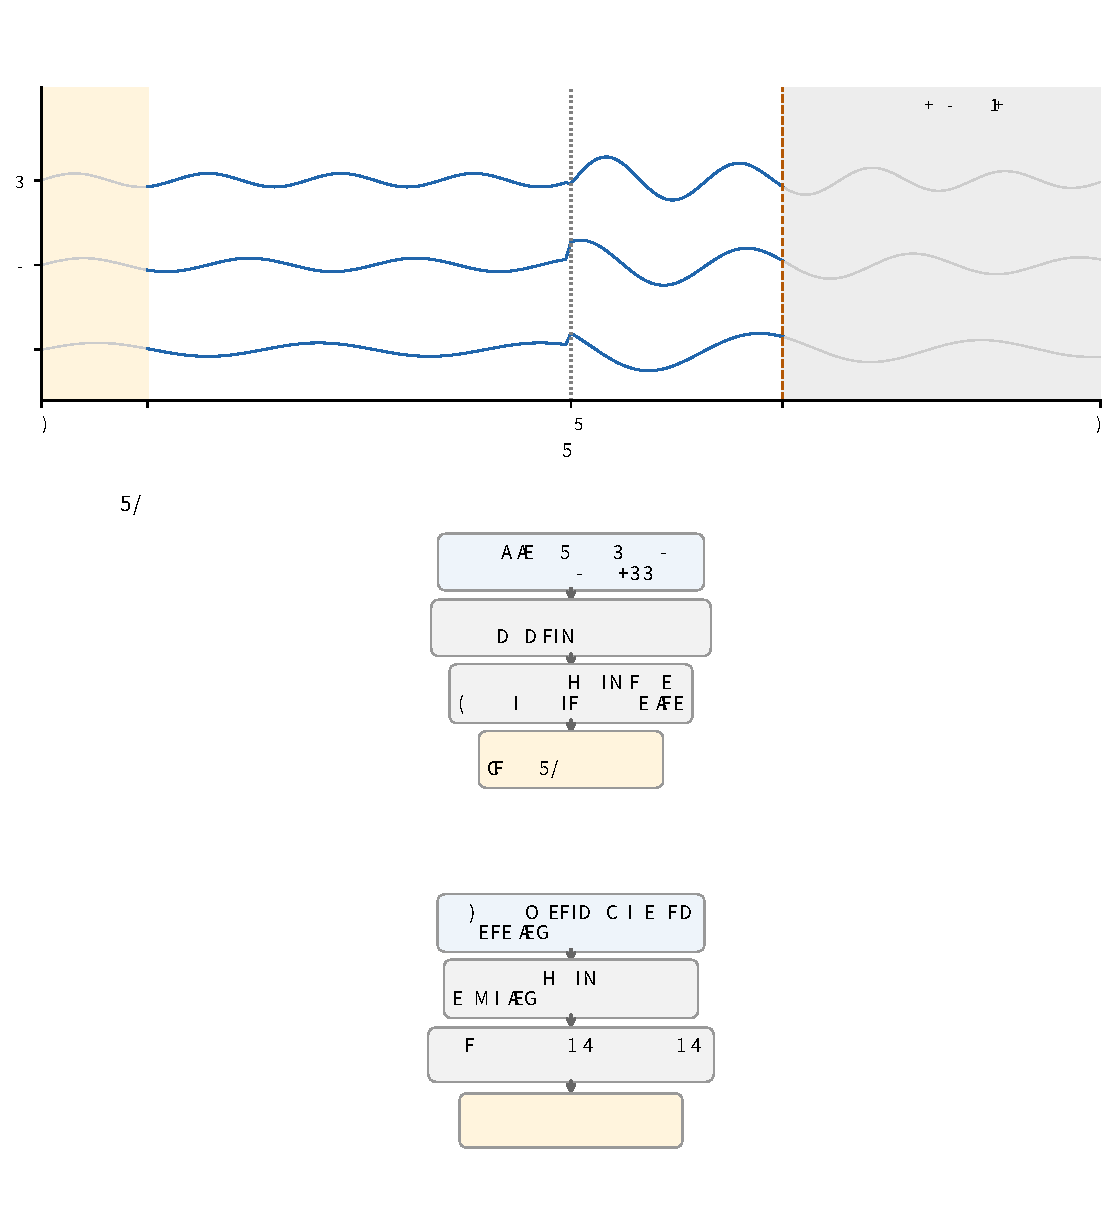
\includegraphics[width=\textwidth,height=.87\textheight,keepaspectratio]{assets/figures/F1.pdf}
\caption{预测任务与模型流程  （a）有效样本读取、掩码、归一化及十一维物理量的处理示意。（b）实际执行的完整 PGA 路径。DiTing、PhaseNet 与 EQTransformer 的波形骨干冻结，适配及读出可训练；TEAM CNN 可训练。台站 memory 直接进入四层目标交叉注意力，当前配置不执行台站上下文自注意力，震级和位置辅助头的预测不回灌 PGA。（c）旧时点动态 noninput 与新固定 never-input 人口，以及三种交付时钟。此图为代码与配置驱动的 SCHEMATIC，不含真实事件波形或性能度量。配置、身份和代码行见 executed\_model\_path.md、F1\_a–c.csv 及输入 manifest。}\end{figure}
\begin{figure}[p]\centering
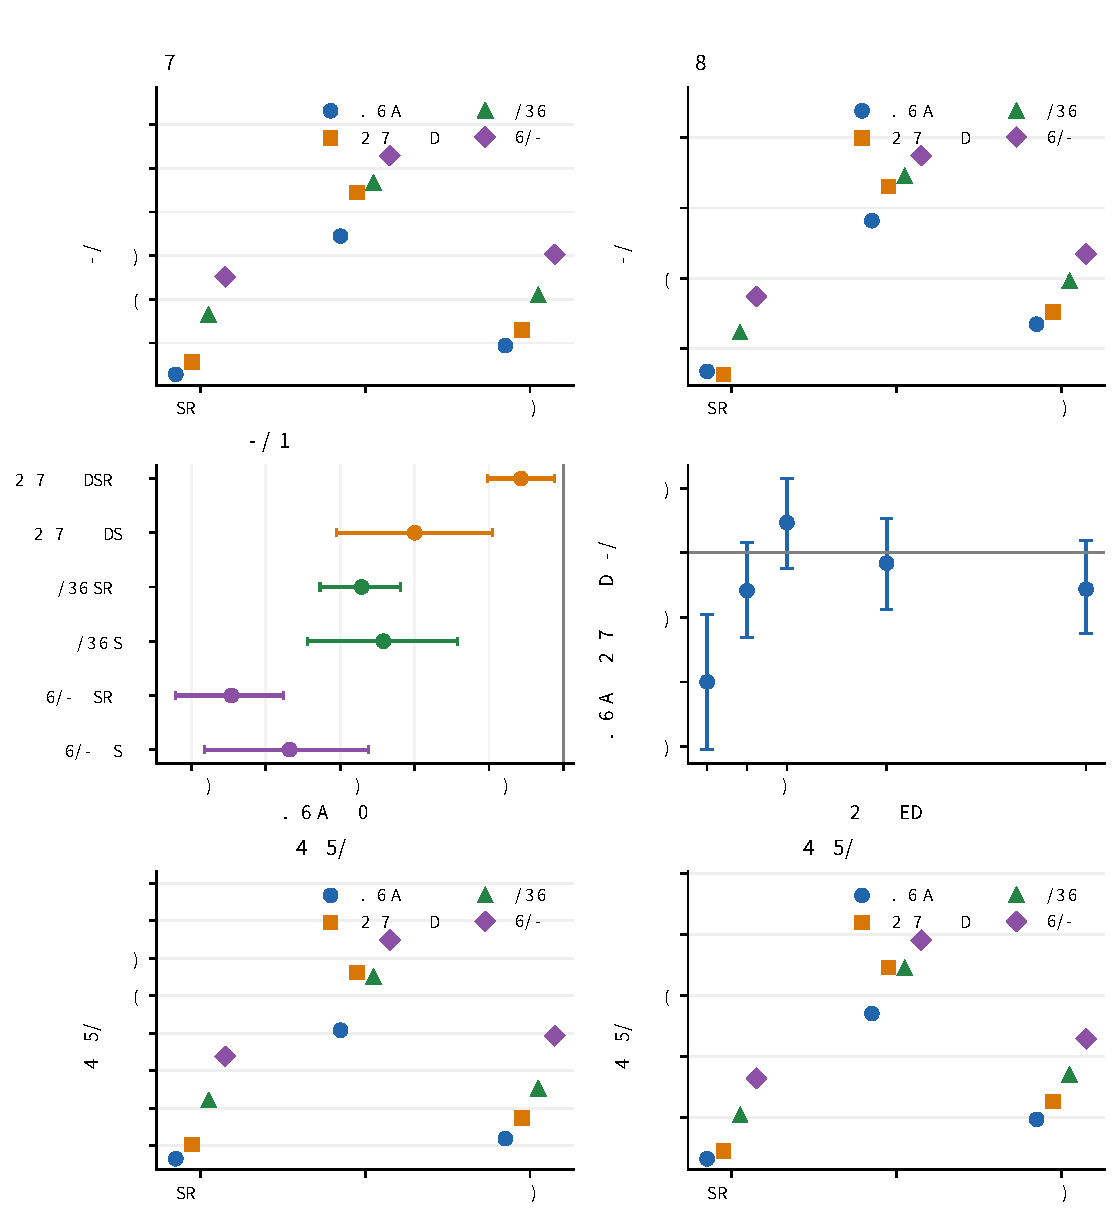
\includegraphics[width=\textwidth,height=.87\textheight,keepaspectratio]{assets/figures/F2.pdf}
\caption{非输入目标预测精度  验证集、seed42，selected 轮次 DiTing/PhaseNet/EQT/TEAM 为 12/12/10/11。主端点为五个共同截止时点与两种几何的十单元，首秒为两个几何单元，早期为 1/3/5 秒六单元。（a、b）非输入与全部目标的 MAE。（c）非输入主端点和首秒的 DiTing 减各参照模型 MAE。（d）DiTing 减 PhaseNet 在五个已有时点的差值，未插值为新逐秒曲线。（e、f）与 a、b 对应的 RMSE，即单元 MSE 等权均值的平方根。误差单位均为 log10(m/s²)，记为 dex；单元内目标等权、单元间等权。c、d 为原有固定模型事件聚类自助法 95\% 区间，2000 次抽样；a、b、e、f 没有伪造绝对指标区间。主端点非输入 1310 事件/139440 请求，全目标 1310/194265；首秒非输入 1310/38795。各早期人口与逐几何支持见 T2 和 F2\_geometry\_time\_support.csv。来源 E03–E07。}\end{figure}
\begin{figure}[p]\centering
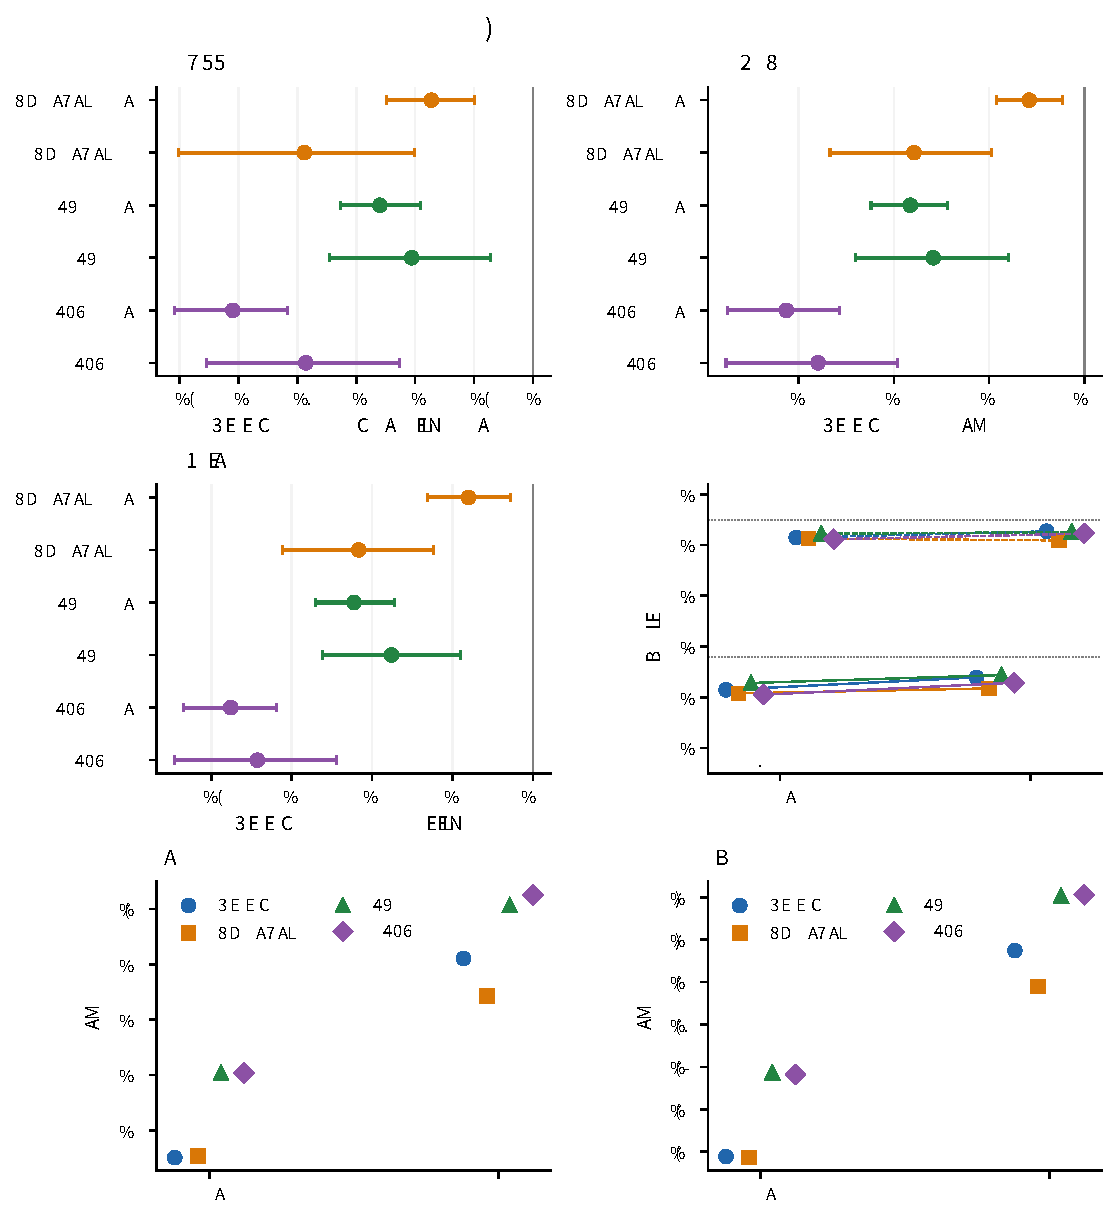
\includegraphics[width=\textwidth,height=.87\textheight,keepaspectratio]{assets/figures/F3.pdf}
\caption{概率预测质量  与图2相同的检查点、验证划分与动态非输入人口。（a–c）主端点和首秒的 NLL、CRPS、Brier 配对差值及原有 95\% 事件聚类区间。NLL 为该 log-PGA 坐标的负对数密度，CRPS 为 dex，Brier 为阈值 −1.2 的无量纲概率平方误差，分轴呈现。（d）68\% 和 95\% 中心区间实际覆盖率，实线与虚线区分名义水平，水平参考线为 0.68/0.95。（e、f）95\% 宽度与预测 sigma，均为 dex。四模型颜色/形状沿用图2，无绝对指标置信区间。较低评分与欠覆盖同时存在，不据覆盖率推造 PIT 或可靠性分箱。全部已保存概率端点见 S3，来源 E03、E04、E07。}\end{figure}
\begin{figure}[p]\centering
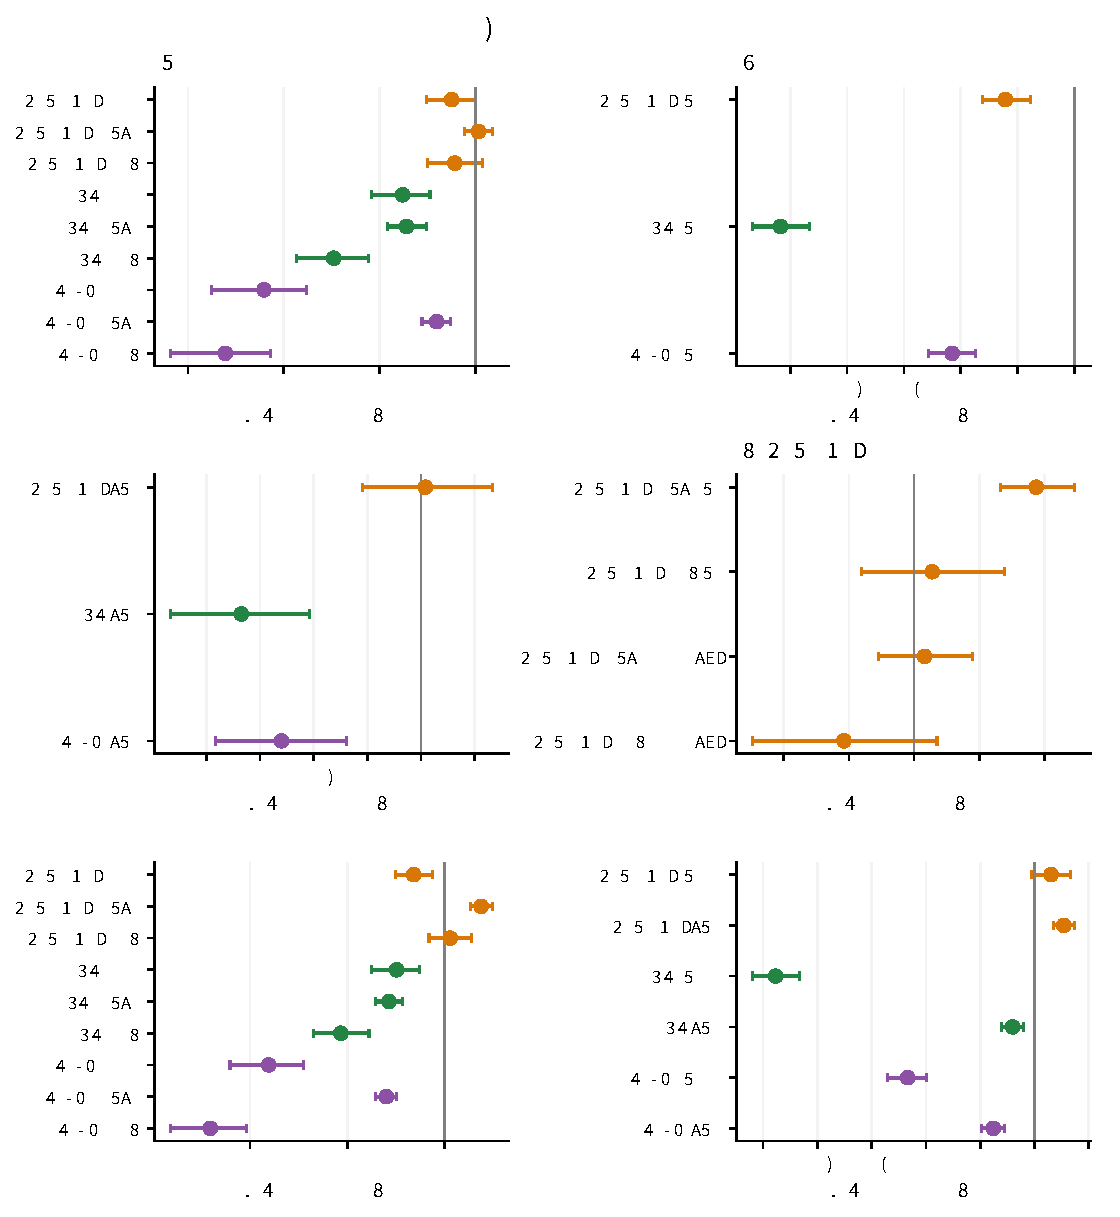
\includegraphics[width=\textwidth,height=.87\textheight,keepaspectratio]{assets/figures/F4.pdf}
\caption{空间预测能力  验证集、seed42、selected 轮次，差值为 DiTing 减参照模型，横线为原有 95\% 事件聚类自助区间。（a–c）非输入目标的 level、shape、field MSE，空间 range 误差及等距对差值误差。（d）PhaseNet 对照下全目标与非输入的 shape/field 对照，保留全目标 shape 的不利结果。（e、f）全目标对所有三种参照模型的 MSE 和 range/pair 对照。MSE 单位为 dex²，range 与 pair 为 dex；PGA 坐标为 log10(m/s²)。各合格场在单元内等权、再对有支持单元等权。非输入 level/shape/field/range 为 944 事件/6789 场，pair 为 928/6644；全目标对应 1057/9250 和 1035/9037。不同空间指标不共享所有分母，K1 等稀疏层只在补充表显示并保留有效重复次数。来源 E08；逐行人口和区间见 F4\_a–f.csv。}\end{figure}
\begin{figure}[p]\centering
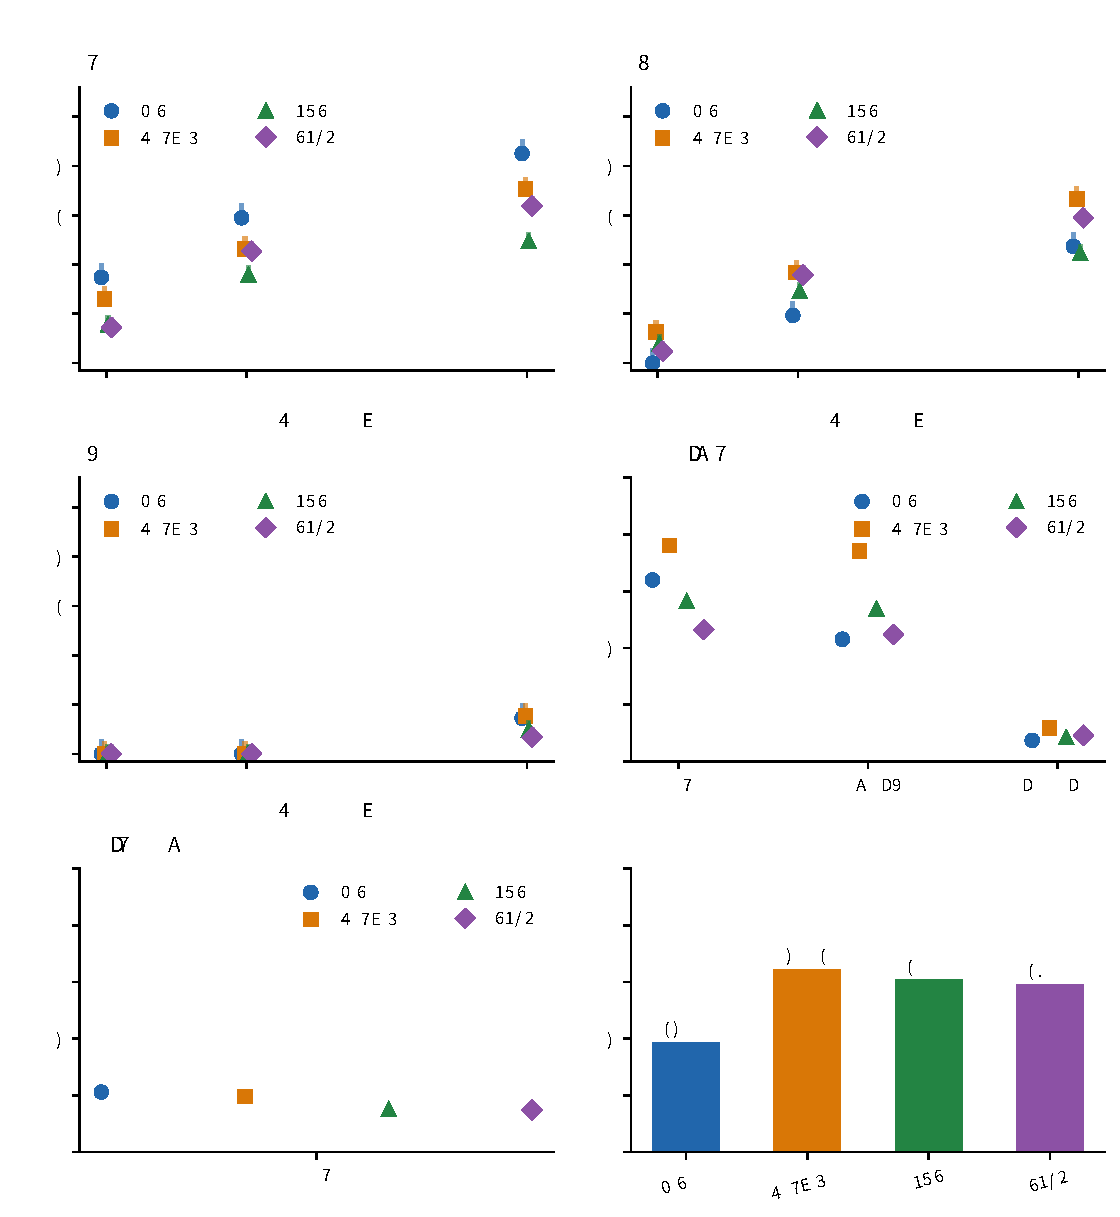
\includegraphics[width=\textwidth,height=.87\textheight,keepaspectratio]{assets/figures/F5.pdf}
\caption{场质量确认与交付时钟  固定 query 逐秒回放、validation、seed42、selected 检查点，预算 0.20 dex，field gate。（a–c）normal never-input 人口在理想截止、完整数值及含共享比较图渲染时钟中，5/10/20 秒内的首次三连续通过帧确认比例。每模型以 207 个适格事件作分母，原始共 1310 事件，另有 1103 事件不足五目标。竖线为加入未知事件的支持上界，点为已确认下界，二者均不是置信区间。（d）normal 全目标在 20 秒的三时钟对照，1057 适格事件。（e）random never-input 539 个适格事件的 20 秒理想场景；数值与渲染未执行，不作外推。（f）normal never-input 理想场景中，确认后再次出现已知不通过帧的事件数/各模型已确认事件数。各模型条件人口不同，无配对因果解释。station gate、全部三预算、三个固定 panel 与已有时钟组合见 S5；配对比例差的统计区间另外保存在 E11，不与 a–c 的未知界限混淆。来源 E10–E13、E28。}\end{figure}
\begin{figure}[p]\centering
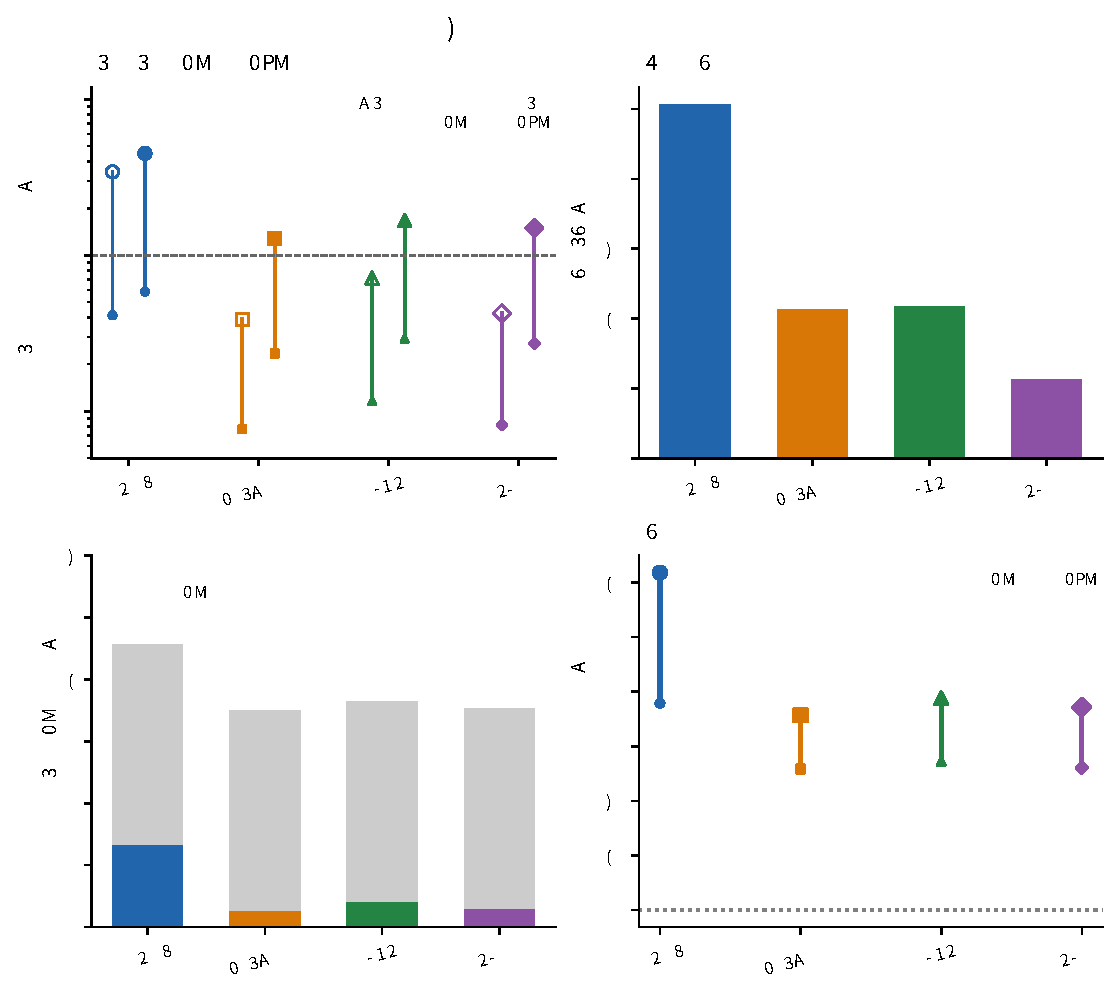
\includegraphics[width=\textwidth,height=.87\textheight,keepaspectratio]{assets/figures/F6.pdf}
\caption{计算时延与交付成本  （a）六事件时延试验的完整 station-only 与 whole-map warm 服务 P50/P95，每范围每模型为 36 帧条件×3 次计时，共 108 次，另有每条件两次预热；空心/实心区分范围，小/大点为 P50/P95，虚线为一秒输入间隔，非统计区间。输入 K 为 1–25，station Q 为 3–80，grid Q 为 1–281。同名设备不能证明严格配对硬件分配。（b）单次 cold-load 单列，起点在 Torch 导入和设备初始化之后，包含认证、读盘、构造与权重加载。（c）全 normal 回放 104800 帧的服务与共享四模型比较图渲染成本 P50；堆叠只展示分项 P50，不能读作总耗时的分位数。（d）首 P 后第 20 秒截止帧的含渲染交付 P50/P95，1310 事件/模型。d 不是 TTUM，a 不是全量回放服务分布，通信仍未测量。含渲染队列的后续 numeric-ready 已受前帧渲染阻塞。全部单位秒。来源 E14–E16。}\end{figure}
\begin{figure}[p]\centering
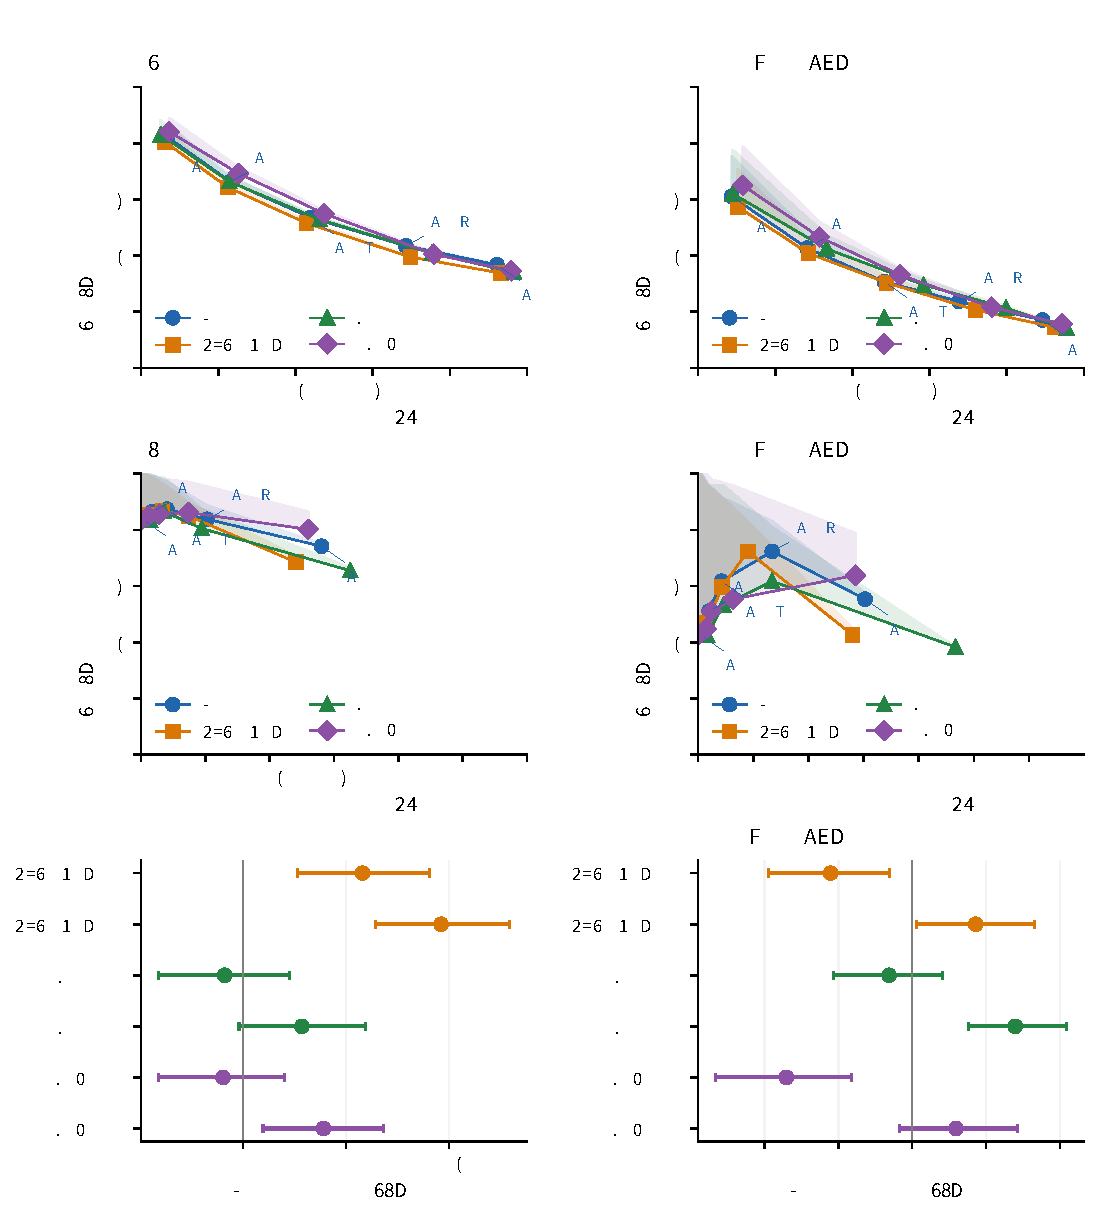
\includegraphics[width=\textwidth,height=.87\textheight,keepaspectratio]{assets/figures/F7.pdf}
\caption{预警失败与误报  normal 固定目标、含渲染时钟、validation、seed42、selected 检查点。（a–d）全目标和 never-input 在 PGA 阈值 −1.2/0.0、提前量至少 3 秒时，受影响目标 pooled 失败下界与完整观测负例 FPR；阴影加入未知后给出上界，均为识别界限而非统计区间。每条曲线包含全部预设告警概率 0.1/0.3/0.5/0.7/0.9；蓝色 DiTing 点标出 p，其他模型按相同概率顺序连接，完整对应表见 source\_data，不按结果选工作点。0.0 与 −1.2 面板的 FPR 显示范围不同，各轴均从零开始。（e、f）阈值 −1.2、p=0.5、tau=3 的事件等权配对差值界及各自 95\% 自助区间，下界为 DiTing 下界减对照上界，上界反之；不是把 pooled 曲线作差，也不是一个确定效应的两个区间。−1.2 全目标原始 1310 事件、1193 个有 affected 的事件、11111 affected 目标；never-input 为 312/214/2336；完整负例分别为 11152 与 2507。该资格不同于图5的至少五目标规则。tau=0/3/5/10 全网格、未知与不完整负例见 S6。来源 E17–E19、E35。}\end{figure}
\clearpage\section*{表格}
\par\textbf{表1 模型与实验设置}\par

\begin{longtable}{llllll}
模型 & 预训练资产 & 骨干状态 & 原生样本数 & 首P后窗能力 s & selected轮次 \\
DiTing & MAE 1200M; corpus/license unresolved & frozen & 10000 & 94.99 & 12 \\
PhaseNet & STEAD v2 & frozen & 3001 & 25.00 & 12 \\
EQT & STEAD v2 & frozen & 6000 & 54.99 & 10 \\
TEAM & scratch & trainable & 10000 & 94.99 & 11 \\
\end{longtable}

\begin{longtable}{llll}
模型 & 总参数 & 可训练参数 & 骨干参数 \\
DiTing & 1280055495 & 46012591 & 1234042904 \\
PhaseNet & 42818657 & 42550214 & 268443 \\
EQT & 42815149 & 42438214 & 376935 \\
TEAM & 48307702 & 48307702 & 5886488 \\
\end{longtable}

四模型均训练12轮、2544更新，seed42；全局批量128、微批量8、Adam学习率0.001、余弦更新调度。前端投影和适配均可训练，共同读出为4层 target cross-attention 加3分量高斯MDN，物理幅值及有效时长共11维。PhaseNet取瓶颈掩码池化与线性投影；EQT取共享CNN/LSTM/Transformer主干后池化投影；DiTing使用归档ViT适配器；TEAM使用可训练CNN。参数量为归档接口审计记录，未在本轮加载权重计数。DiTing精确预训练语料/论文/许可尚未解决。原生窗能力不代表已测长时间性能。来源 metadata/checkpoint\_inventory 与 evidence/complete\_model\_settings.json。
\par\textbf{表2 主要预测结果}\par

validation，seed42，selected轮次按表1。误差坐标为log10(m/s²)，记为dex；除明确pooled栏外，单元内请求等权、单元间等权。RMSE为等单元MSE开方。Brier阈值−1.2；覆盖率为比例；NLL为负对数密度。为保证可读性，表2分点误差、概率评分和校准子表；每个端点与人口分别成块，不能跨块合并样本。

\par\textbf{十单元主端点 非输入目标}\par

政策 selected，轮次依次12/12/10/11；1310事件，139440请求，10单元。

\begin{longtable}{llll}
模型 & MAE dex & RMSE dex & bias dex \\
DiTing & 0.222859 & 0.296500 & 0.000138 \\
PhaseNet & 0.225697 & 0.300372 & -0.009276 \\
EQT & 0.236407 & 0.312033 & -0.000829 \\
TEAM & 0.245159 & 0.323800 & 0.002668 \\
\end{longtable}

\begin{longtable}{llll}
模型 & NLL & CRPS dex & Brier \\
DiTing & 0.115770 & 0.159220 & 0.169824 \\
PhaseNet & 0.150267 & 0.162109 & 0.173825 \\
EQT & 0.167722 & 0.168356 & 0.180948 \\
TEAM & 0.217655 & 0.174864 & 0.188617 \\
\end{longtable}

\begin{longtable}{lllll}
模型 & 覆盖68 & 覆盖95 & 宽度95 dex & sigma dex \\
DiTing & 0.614525 & 0.914884 & 0.975356 & 0.248804 \\
PhaseNet & 0.607498 & 0.913038 & 0.976773 & 0.248571 \\
EQT & 0.628063 & 0.922287 & 1.051932 & 0.268578 \\
TEAM & 0.605038 & 0.911661 & 1.051705 & 0.268215 \\
\end{longtable}


\par\textbf{十单元主端点 全部目标}\par

政策 selected，轮次依次12/12/10/11；1310事件，194265请求，10单元。

\begin{longtable}{llll}
模型 & MAE dex & RMSE dex & bias dex \\
DiTing & 0.213540 & 0.286397 & -0.010688 \\
PhaseNet & 0.212698 & 0.288894 & -0.021052 \\
EQT & 0.224523 & 0.300616 & -0.022248 \\
TEAM & 0.234851 & 0.312822 & -0.012400 \\
\end{longtable}

\begin{longtable}{llll}
模型 & NLL & CRPS dex & Brier \\
DiTing & 0.059612 & 0.152538 & 0.161636 \\
PhaseNet & 0.042111 & 0.152456 & 0.162063 \\
EQT & 0.098654 & 0.160037 & 0.170253 \\
TEAM & 0.165417 & 0.167804 & 0.179313 \\
\end{longtable}

\begin{longtable}{lllll}
模型 & 覆盖68 & 覆盖95 & 宽度95 dex & sigma dex \\
DiTing & 0.624168 & 0.921673 & 0.952025 & 0.242751 \\
PhaseNet & 0.623204 & 0.921796 & 0.943944 & 0.239425 \\
EQT & 0.638686 & 0.929097 & 1.016717 & 0.259096 \\
TEAM & 0.615093 & 0.918240 & 1.026353 & 0.261477 \\
\end{longtable}


\par\textbf{首秒两单元 非输入目标}\par

政策 selected，轮次依次12/12/10/11；1310事件，38795请求，2单元。

\begin{longtable}{llll}
模型 & MAE dex & RMSE dex & bias dex \\
DiTing & 0.254466 & 0.330788 & -0.012768 \\
PhaseNet & 0.264456 & 0.346155 & -0.039416 \\
EQT & 0.266558 & 0.345052 & -0.008028 \\
TEAM & 0.272866 & 0.354810 & -0.030629 \\
\end{longtable}

\begin{longtable}{llll}
模型 & NLL & CRPS dex & Brier \\
DiTing & 0.255935 & 0.180840 & 0.198390 \\
PhaseNet & 0.333513 & 0.189780 & 0.209229 \\
EQT & 0.297069 & 0.188773 & 0.207183 \\
TEAM & 0.333021 & 0.194823 & 0.215531 \\
\end{longtable}

\begin{longtable}{lllll}
模型 & 覆盖68 & 覆盖95 & 宽度95 dex & sigma dex \\
DiTing & 0.639177 & 0.927402 & 1.155329 & 0.297441 \\
PhaseNet & 0.617423 & 0.908934 & 1.121388 & 0.288937 \\
EQT & 0.643737 & 0.926084 & 1.203378 & 0.310322 \\
TEAM & 0.628562 & 0.922933 & 1.212905 & 0.310597 \\
\end{longtable}


\par\textbf{首秒两单元 全部目标}\par

政策 selected，轮次依次12/12/10/11；1310事件，41898请求，2单元。

\begin{longtable}{llll}
模型 & MAE dex & RMSE dex & bias dex \\
DiTing & 0.256346 & 0.334057 & -0.023718 \\
PhaseNet & 0.266073 & 0.349115 & -0.048787 \\
EQT & 0.268994 & 0.348847 & -0.021693 \\
TEAM & 0.274844 & 0.358130 & -0.042672 \\
\end{longtable}

\begin{longtable}{llll}
模型 & NLL & CRPS dex & Brier \\
DiTing & 0.266131 & 0.182670 & 0.197622 \\
PhaseNet & 0.341933 & 0.191382 & 0.207740 \\
EQT & 0.310647 & 0.191107 & 0.206993 \\
TEAM & 0.344991 & 0.196847 & 0.214518 \\
\end{longtable}

\begin{longtable}{lllll}
模型 & 覆盖68 & 覆盖95 & 宽度95 dex & sigma dex \\
DiTing & 0.635076 & 0.925809 & 1.150763 & 0.296093 \\
PhaseNet & 0.615146 & 0.907824 & 1.118777 & 0.288110 \\
EQT & 0.638447 & 0.923772 & 1.198424 & 0.308850 \\
TEAM & 0.623557 & 0.921269 & 1.206761 & 0.308857 \\
\end{longtable}


\par\textbf{早期六单元 非输入目标}\par

政策 selected，轮次依次12/12/10/11；1310事件，98889请求，6单元。

\begin{longtable}{llll}
模型 & MAE dex & RMSE dex & bias dex \\
DiTing & 0.229410 & 0.301865 & 0.002081 \\
PhaseNet & 0.232938 & 0.307448 & -0.011204 \\
EQT & 0.240957 & 0.315175 & 0.001311 \\
TEAM & 0.250303 & 0.329313 & -0.007841 \\
\end{longtable}

\begin{longtable}{llll}
模型 & NLL & CRPS dex & Brier \\
DiTing & 0.136191 & 0.162910 & 0.176004 \\
PhaseNet & 0.168167 & 0.166240 & 0.180643 \\
EQT & 0.176981 & 0.170455 & 0.184939 \\
TEAM & 0.231953 & 0.178091 & 0.193659 \\
\end{longtable}

\begin{longtable}{lllll}
模型 & 覆盖68 & 覆盖95 & 宽度95 dex & sigma dex \\
DiTing & 0.627334 & 0.921424 & 1.024529 & 0.262512 \\
PhaseNet & 0.615518 & 0.913675 & 1.003257 & 0.256944 \\
EQT & 0.641910 & 0.928785 & 1.092010 & 0.280371 \\
TEAM & 0.618102 & 0.919185 & 1.099997 & 0.281059 \\
\end{longtable}


\par\textbf{早期六单元 全部目标}\par

政策 selected，轮次依次12/12/10/11；1310事件，119983请求，6单元。

\begin{longtable}{llll}
模型 & MAE dex & RMSE dex & bias dex \\
DiTing & 0.226951 & 0.299349 & -0.010224 \\
PhaseNet & 0.230428 & 0.305183 & -0.022288 \\
EQT & 0.239101 & 0.313811 & -0.017423 \\
TEAM & 0.246894 & 0.325799 & -0.023053 \\
\end{longtable}

\begin{longtable}{llll}
模型 & NLL & CRPS dex & Brier \\
DiTing & 0.127564 & 0.161518 & 0.172731 \\
PhaseNet & 0.155334 & 0.164710 & 0.176798 \\
EQT & 0.171798 & 0.169648 & 0.182235 \\
TEAM & 0.221729 & 0.176280 & 0.189418 \\
\end{longtable}

\begin{longtable}{lllll}
模型 & 覆盖68 & 覆盖95 & 宽度95 dex & sigma dex \\
DiTing & 0.627866 & 0.923237 & 1.014141 & 0.259636 \\
PhaseNet & 0.617748 & 0.916356 & 0.995661 & 0.254742 \\
EQT & 0.640733 & 0.929461 & 1.079528 & 0.276843 \\
TEAM & 0.618787 & 0.921004 & 1.085756 & 0.277123 \\
\end{longtable}

\par\textbf{合并请求伴随统计}\par

以下仅列非输入主端点，其余在T2\_pooled.csv。R²和斜率按合并请求计算，不是等单元统计。

\begin{longtable}{llll}
模型 & pooled请求 & pooled R² & 预测对真值斜率 \\
DiTing & 139440 & 0.432956 & 0.480508 \\
PhaseNet & 139440 & 0.412157 & 0.447309 \\
EQT & 139440 & 0.377906 & 0.416067 \\
TEAM & 139440 & 0.329485 & 0.380688 \\
\end{longtable}
\par\textbf{表3 评价人口与支持范围}\par

旧协议请求/新固定目标/空间场/预警受影响目标分别统计；TTUM与shadow资格不同。图5 unknown为事件数，图7 unknown为受影响目标数。下表不据未执行时钟组合填值。

未知数以DiTing为例，其他模型见S5/S6；人口分母为共同支持。

shadow行的事件子集列指含受影响目标的事件，误报另用完整负例分母。

\begin{longtable}{lllllll}
协议 & 人口 & 原始事件 & 可评价事件 & 不适格事件 & 请求/场/目标 & 未知 \\
旧五时点×两几何 & 全部 & 1310 & 1310 & 0 & 194265 & 无失败请求 \\
旧五时点×两几何 & 逐时点非输入 & 1310 & 1310 & 0 & 139440 & 无失败请求 \\
固定目标 normal & 固定全部 & 1310 & 1057 & 253 & 固定目标见S5 & 27 \\
固定目标 normal & 固定never-input & 1310 & 207 & 1103 & 固定目标见S5 & 6 \\
固定目标 random & 固定全部 & 1310 & 1057 & 253 & 固定目标见S5 & 15 \\
固定目标 random & 固定never-input & 1310 & 539 & 771 & 固定目标见S5 & 3 \\
失败 normal渲染 −1.2 p.5 tau3 & 固定全部 & 1310 & 1193 & 不适用 & 11111 & 83 \\
失败 normal渲染 −1.2 p.5 tau3 & 固定never-input & 312 & 214 & 不适用 & 2336 & 49 \\
\end{longtable}

旧协议为cutoff时钟；固定query normal有ideal/numeric/rendered，random只有ideal；shadow正文采用normal rendered。空间非输入944事件/6789场（pair为928/6644），全目标1057/9250（pair为1035/9037）。六事件计时每模型每scope108次，与全normal104800帧服务统计分开。缺失预测、资格不足和未知结局在各自原表保留，不删除后计算成功率。
\end{document}
